% !TeX root = main.tex

\chapter{Implementation Results and Discussion}
\label{chap:results}

This chapter presents the culminating results of the thesis, transitioning from theoretical design to tangible implementation and empirical validation. The System-on-Chip (SoC), designed programmatically in Chisel, was compiled through the FIRRTL intermediate representation and subsequently implemented using the Xilinx Vivado toolchain for the VC707 FPGA target. This chapter is organized into three main sections. First, it details the hardware implementation results, including the final system architecture and an analysis of on-chip resource utilization and power consumption. Second, it documents the successful deployment of the full software stack, demonstrating a boot-to-Linux environment. Finally, and most critically, it evaluates the performance of the integrated Gemmini DNN accelerator, providing quantitative evidence of its effectiveness.

\section{Hardware Implementation Analysis}
\label{sec:hardware_results}

The hardware generation process produces a set of Verilog files that are synthesized, placed, and routed by the Vivado Design Suite. The following sections analyze the final hardware implementation from architectural, resource, and power perspectives.

\subsection{System Block Design and Address Map}

The generated system is a complex integration of the RISC-V core, the Gemmini accelerator, memory subsystems, and peripherals. The block diagrams in Figure \ref{fig:block_design}, Figure \ref{fig:block_design_ddr}, and Figure \ref{fig:block_design_io} provide a visual representation of the final hardware architecture as implemented in Vivado. These diagrams confirm the successful integration of all system components, from the top-level SoC (Figure \ref{fig:block_design}) down to the specific connections for DDR memory (Figure \ref{fig:block_design_ddr}) and I/O peripherals like UART and Ethernet (Figure \ref{fig:block_design_io}).

The system's memory-mapped architecture is confirmed by the Address Editor view in Figure \ref{fig:address_editor}, which shows the memory ranges assigned to the DDR memory controller, the Gemmini DMA interface, and various peripheral buses. This confirms that the diplomacy framework within Chipyard correctly generated the necessary hardware and address decoding logic.

\begin{figure}[h!]
\centering
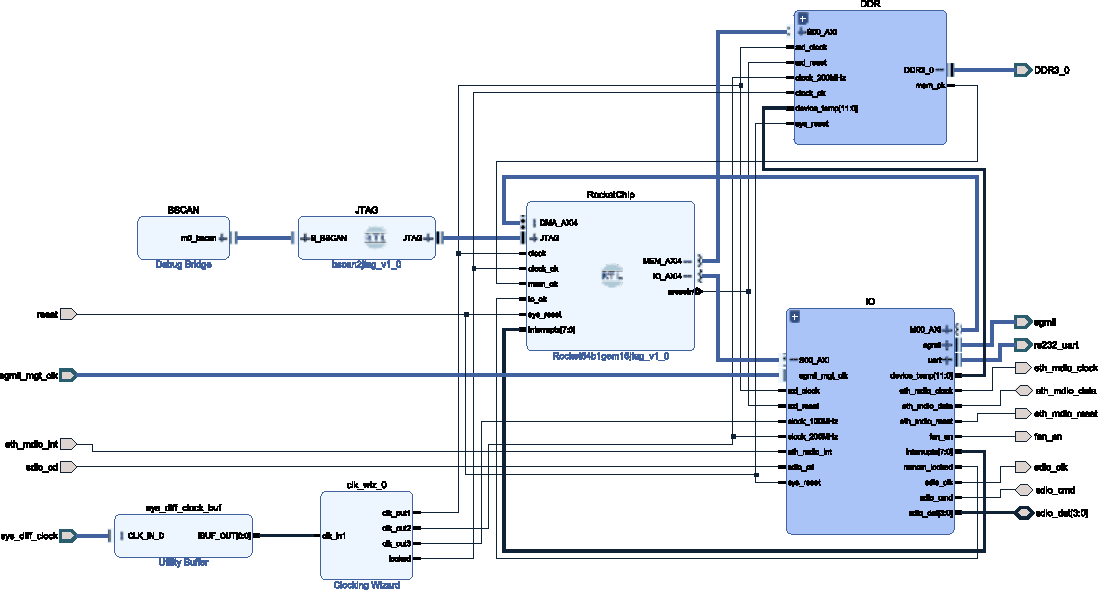
\includegraphics[width=\textwidth]{Images/Results/BlockDesign_System.pdf}
\caption{Block Design of the System, showing the top-level integration of the RocketChip core, DDR, and IO subsystems.}
\label{fig:block_design}
\end{figure}

\begin{figure}[h!]
\centering
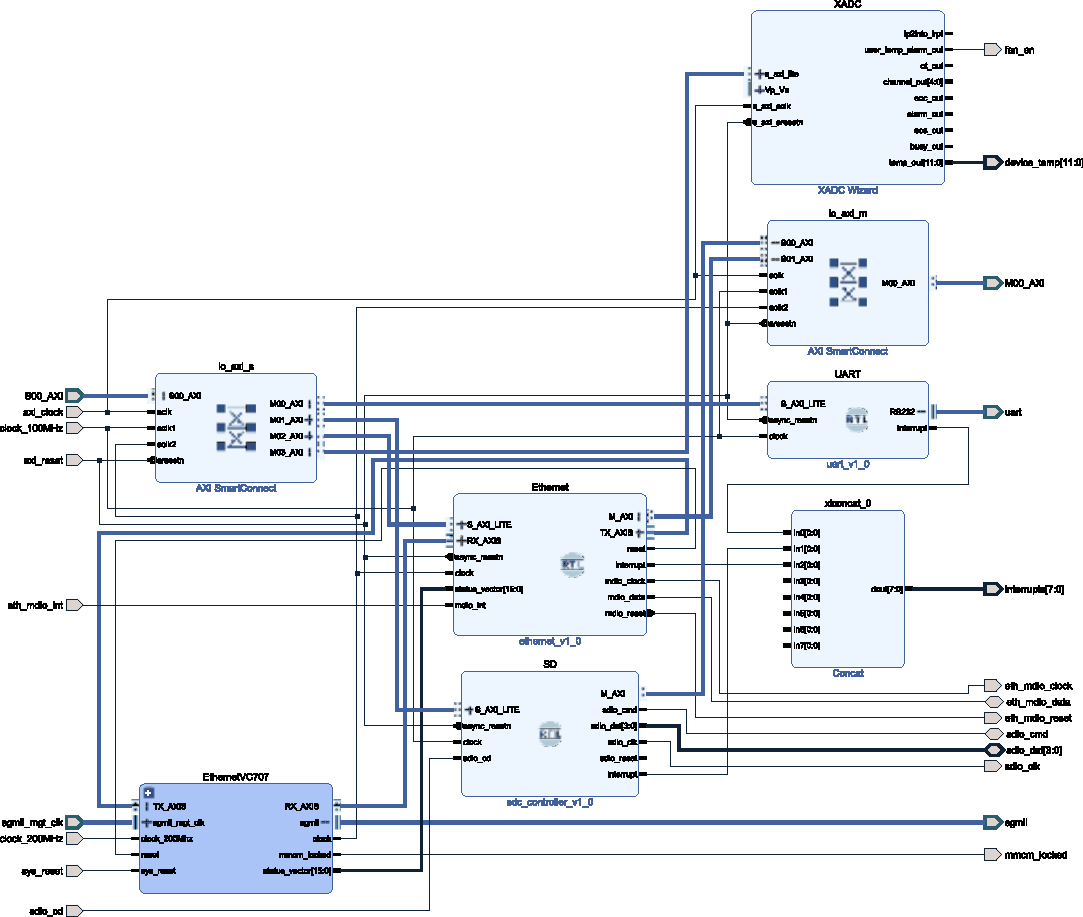
\includegraphics[width=\textwidth]{Images/Results/BlockDesign_IO.pdf}
\caption{Block Design of the IO Subsystem, illustrating the AXI interconnect for peripherals such as Ethernet, SD Card, and UART.}
\label{fig:block_design_io}
\end{figure}

\begin{figure}[h!]
\centering
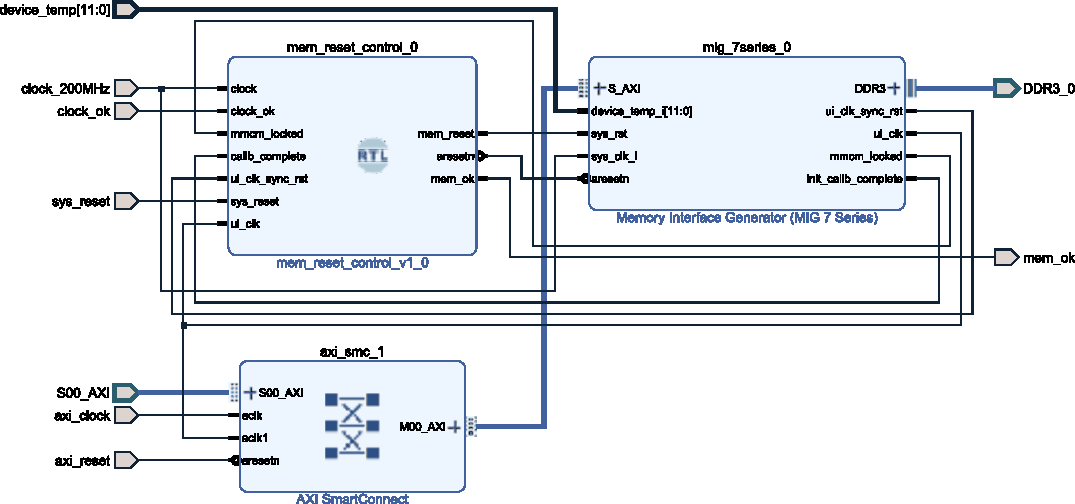
\includegraphics[width=0.8\textwidth]{Images/Results/BlockDesign_DDR.pdf}
\caption{Block Design of the DDR Subsystem, detailing the Memory Interface Generator (MIG) and its AXI connection.}
\label{fig:block_design_ddr}
\end{figure}

\begin{figure}[h!]
\centering
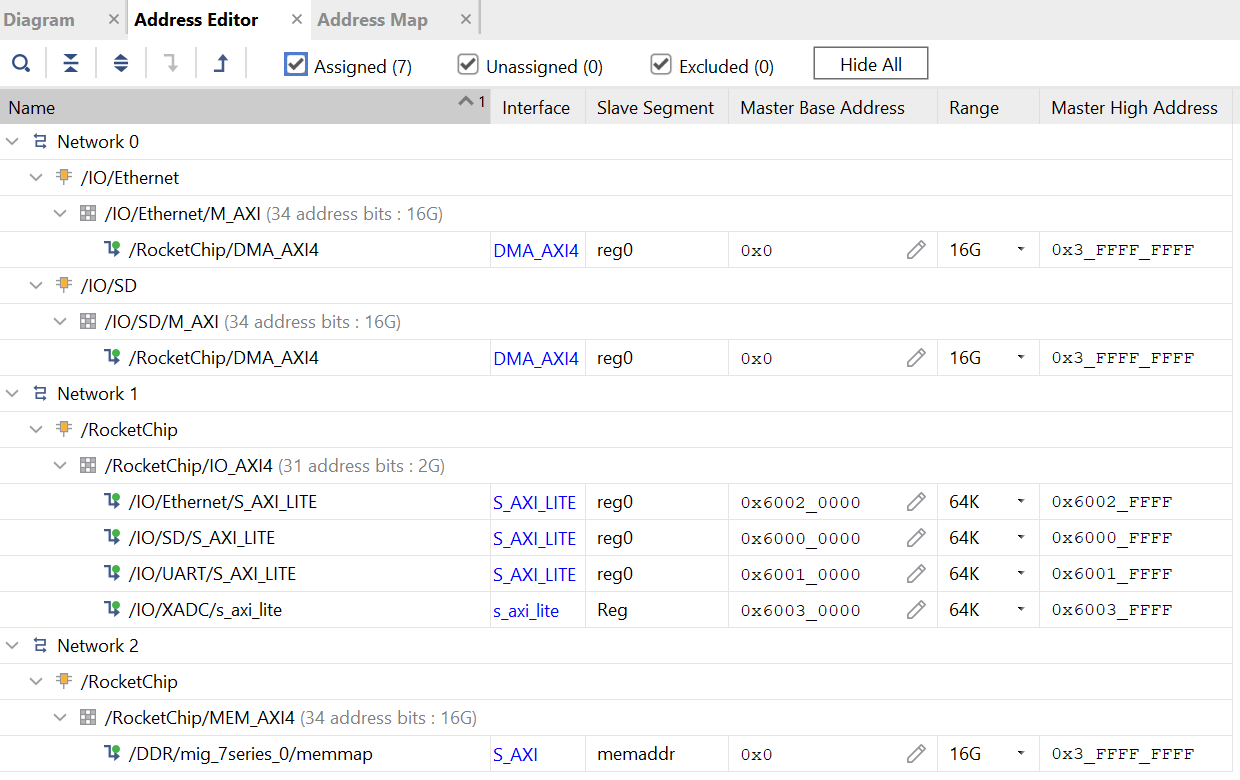
\includegraphics[width=0.8\textwidth]{Images/Results/AddressEditor}
\caption{Address Editor view, confirming the memory map for the integrated peripherals.}
\label{fig:address_editor}
\end{figure}

\subsection{Vivado Implemented Design Results}

\subsubsection{Device Utilization Analysis}
Resource utilization is a critical metric for evaluating the cost and feasibility of an SoC implementation on a given FPGA. The post-implementation utilization report from Vivado provides a detailed accounting of the hardware resources consumed by the design.

As shown in Figure \ref{fig:utilization_summary_detailed}, the complete, Linux-capable SoC is a substantial design, consuming \textbf{80.92\%} of the available Look-Up Tables (LUTs), \textbf{28.59\%} of Block RAM (BRAM), and \textbf{8.96\%} of DSP slices on the Xilinx VC707's Virtex-7 FPGA. The high LUT utilization is expected given the complexity of a 64-bit processor core with an L2 cache and numerous peripherals. The significant BRAM usage is primarily attributable to the memory-intensive components of the design, namely the L2 cache and the Gemmini accelerator's scratchpad and accumulator memories.

To isolate the resource cost of the Gemmini accelerator itself, a hierarchical utilization analysis was performed. Figure \ref{fig:utilization_hierarchical_gemmini} shows that the Gemmini module (`riscv\_tile/riscv\_tile/Queue\_Gemmini`) consumes 180,142 LUTs. This represents approximately 73.5\% of the logic within the `riscv\_tile` and underscores the fact that the specialized accelerator is, by far, the largest single component in the processor tile, dwarfing the RISC-V core itself. This trade-off of silicon area for specialized performance is the central premise of hardware acceleration.

% \begin{figure}[h!]
% \centering
% 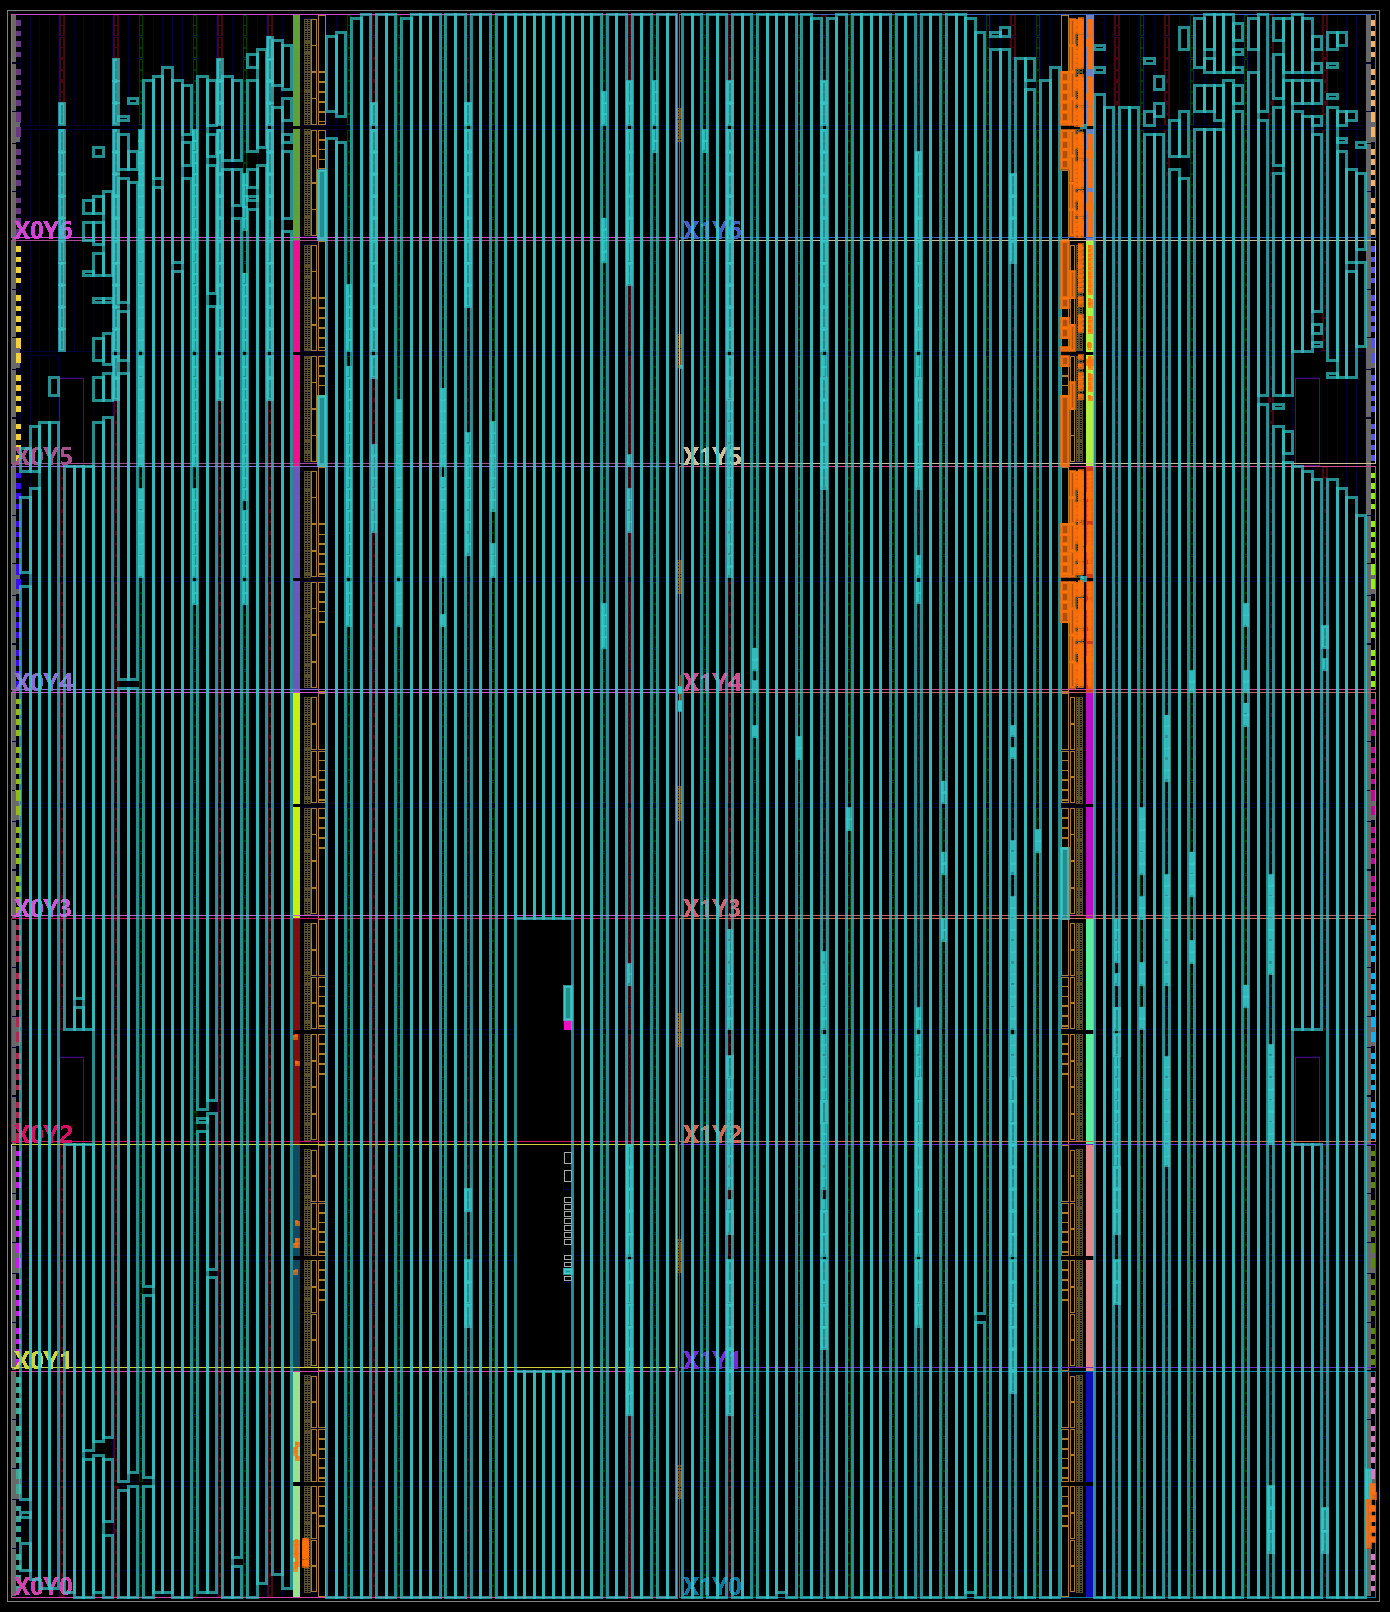
\includegraphics[width=\textwidth]{Images/Results/DeviceView}
% \caption{Device View of the implemented design on the FPGA fabric.}
% \label{fig:device_view}
% \end{figure}

\begin{figure}[h!]
\centering
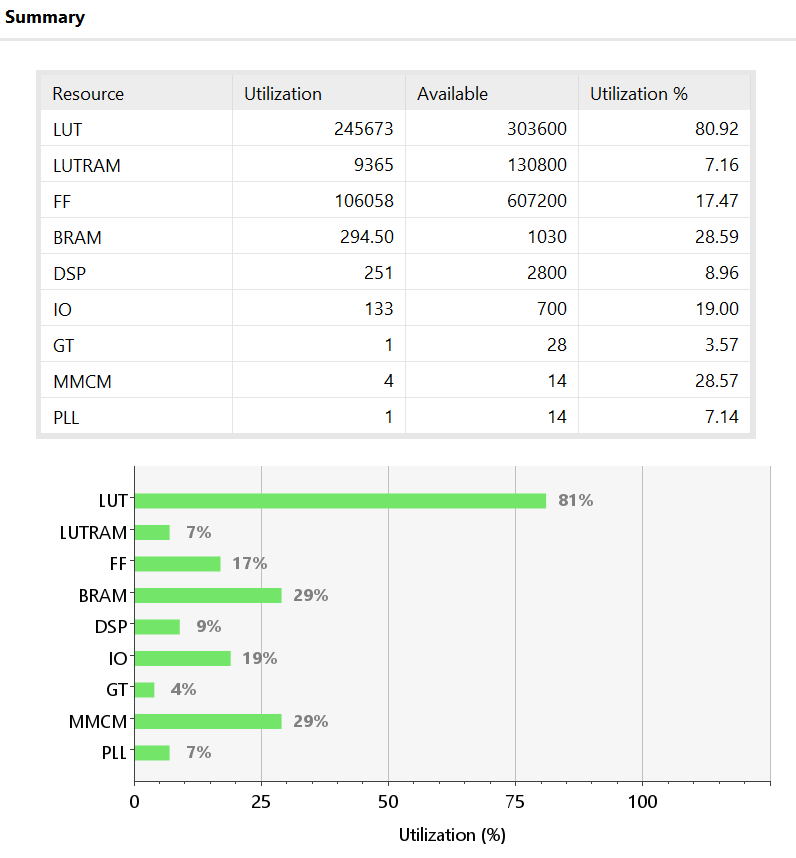
\includegraphics[width=\textwidth]{Images/Results/Utilization_Summary_Detailed.png}
\caption{Detailed Utilization Summary for the entire SoC on the VC707 FPGA.}
\label{fig:utilization_summary_detailed}
\end{figure}

% \begin{figure}[h!]
% \centering
% 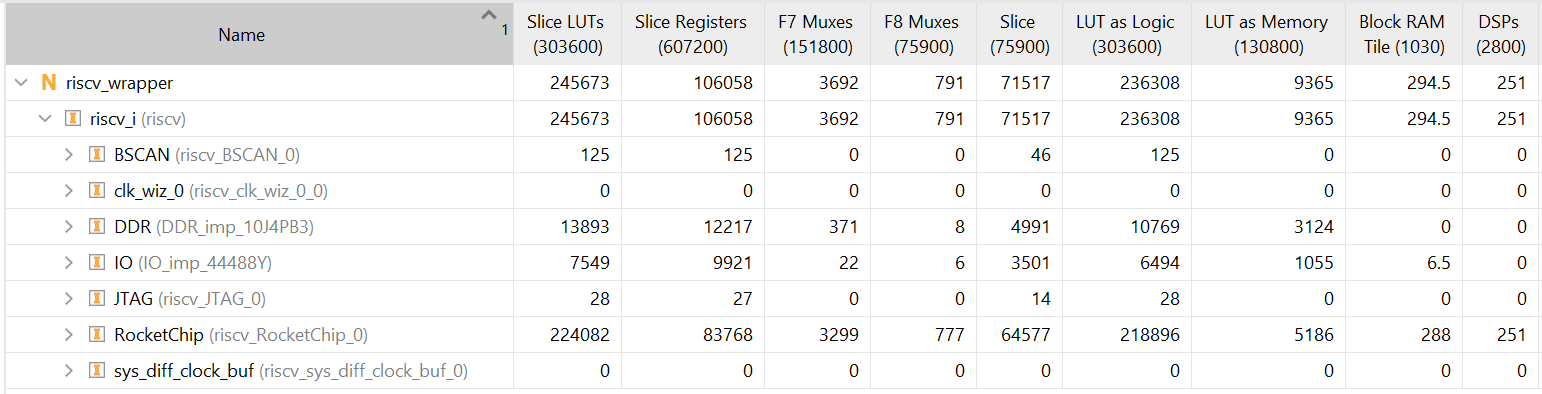
\includegraphics[width=\textwidth]{Images/Results/Utilization_Hierarchical.png}
% \caption{Hierarchical Utilization, showing the breakdown of resources by major system modules.}
% \label{fig:utilization_hierarchical}
% \end{figure}

\begin{figure}[h!]
\centering
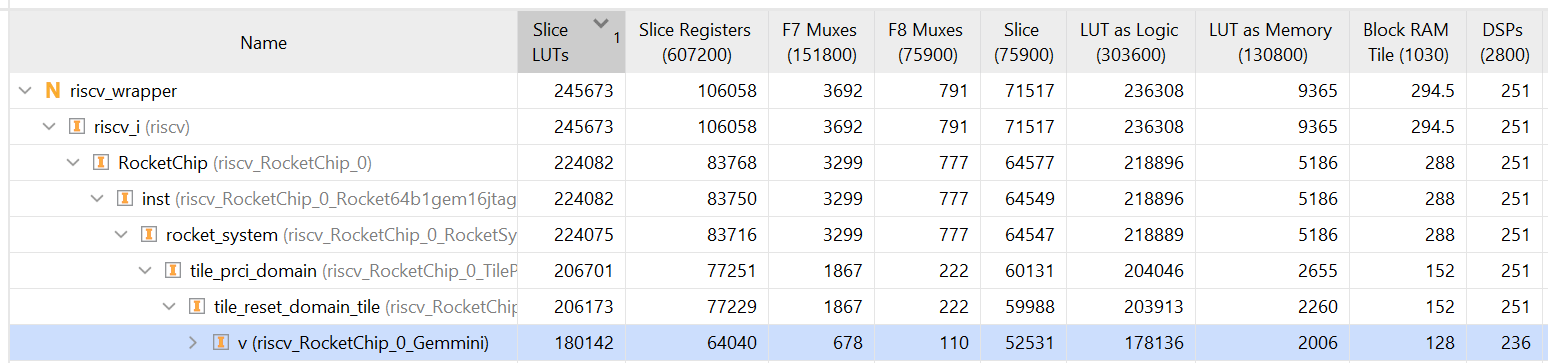
\includegraphics[width=\textwidth]{Images/Results/Utilization_Hierarchical_Gemmini.png}
\caption{Hierarchical Utilization of the Gemmini accelerator module.}
\label{fig:utilization_hierarchical_gemmini}
\end{figure}


\subsubsection{Power Consumption Analysis}

Power analysis, performed by Vivado based on the placed-and-routed design and simulation-derived activity factors, is crucial for understanding the thermal and power-delivery requirements of the system.

The power summary in Figure \ref{fig:power_summary} reports a \textbf{Total On-Chip Power of 3.856W}. A key observation is the breakdown between static and dynamic power. Dynamic power, consumed by switching logic, accounts for 3.309W (86\% of the total), while static power is only 0.237W (6\%). This is characteristic of a high-performance digital design where power consumption is dominated by computational activity rather than leakage. The report identifies that the most significant contributors to dynamic power are Clocks, Signals, and I/O, which is expected for a large, high-frequency SoC with multiple external interfaces. The power hierarchical report (Figure \ref{fig:power_hierarchical_gemmini}) further shows that the Gemmini module contributes significantly to the overall power budget, consistent with its large area and high level of computational activity.

% \begin{figure}[h!]
% \centering
% 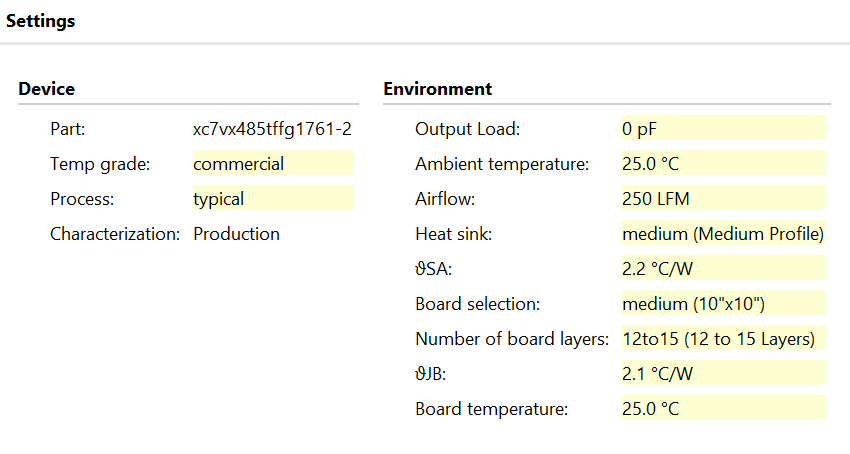
\includegraphics[width=\textwidth]{Images/Results/Power_Settings.png}
% \caption{Power analysis settings.}
% \label{fig:power_settings}
% \end{figure}

% \begin{figure}[h!]
% \centering
% 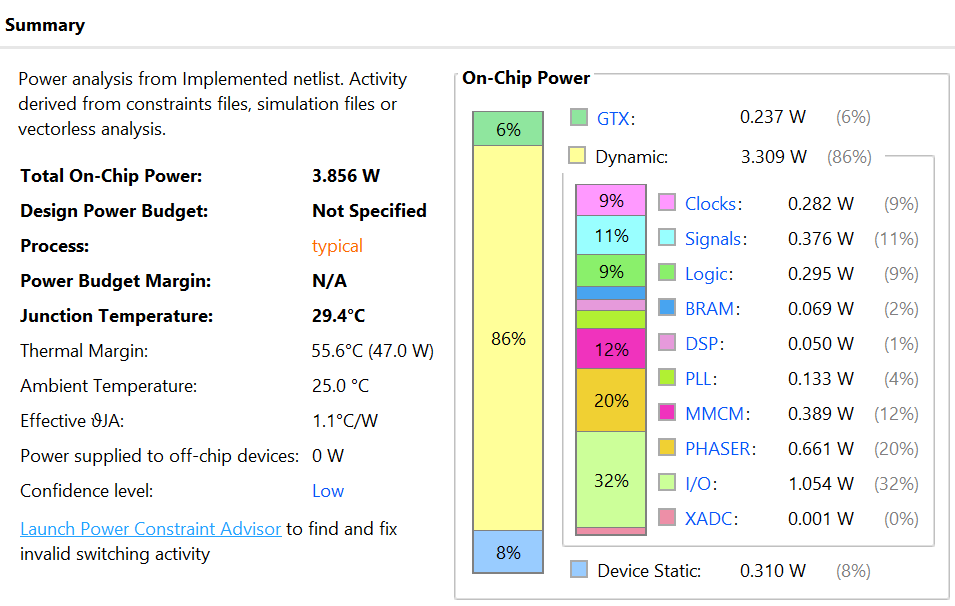
\includegraphics[width=\textwidth]{Images/Results/Power_Summary.png}
% \caption{Post-implementation on-chip power summary.}
% \label{fig:power_summary}
% \end{figure}

% \begin{figure}[h!]
% \centering
% 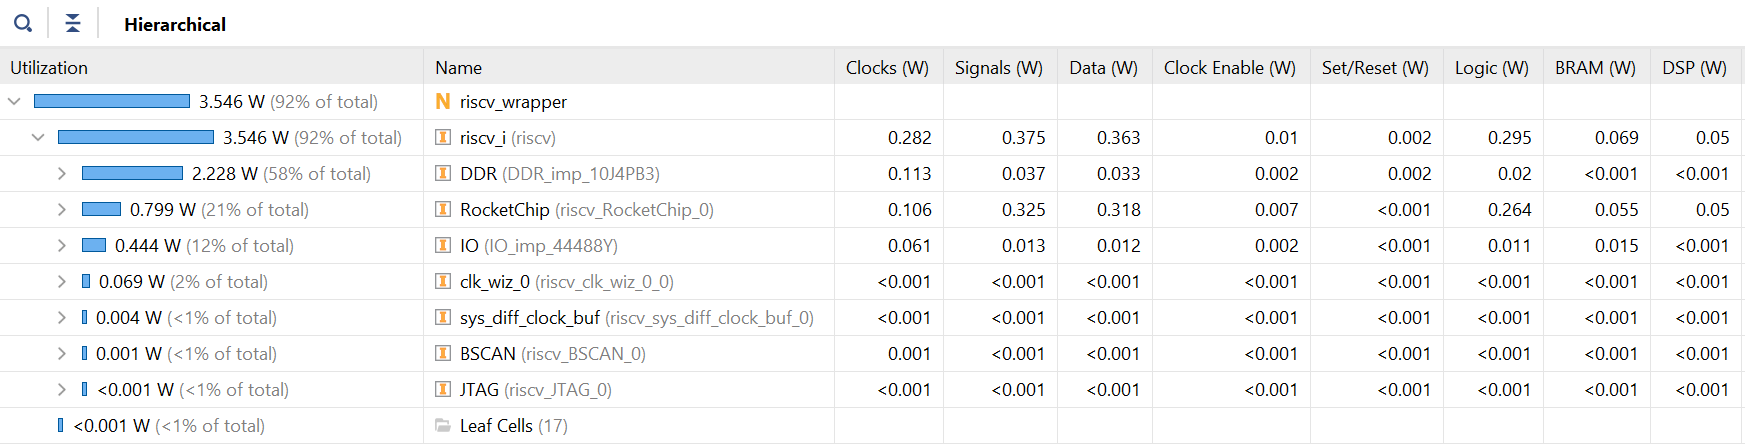
\includegraphics[width=\textwidth]{Images/Results/Power_Hierarchical.png}
% \caption{Hierarchical power report for the entire system.}
% \label{fig:power_hierarchical}
% \end{figure}

\begin{figure}[h!]
\centering
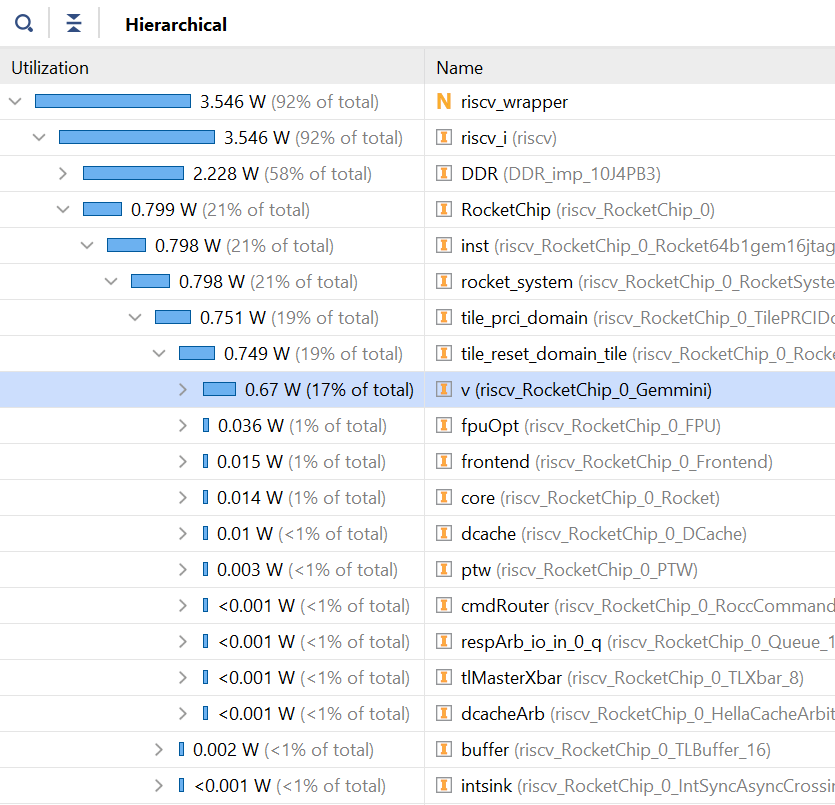
\includegraphics[width=\textwidth]{Images/Results/Power_Hierarchical_Gemmini.png}
\caption{Hierarchical power report for the Gemmini accelerator.}
\label{fig:power_hierarchical_gemmini}
\end{figure}

\FloatBarrier

\section{Software Stack Validation}
\label{sec:software_results}
A primary objective of this thesis was to implement a full-stack, Linux-capable system. This section provides evidence of this successful implementation by documenting the complete boot process, from the initial on-chip Boot ROM to a fully functional Debian Linux user environment.

\subsection{System Boot Sequence}
The system boot process involves a multi-stage software chain, starting with the first-stage bootloader in ROM, which then loads subsequent stages from the SD card. The console output in Listing \ref{lst:boot_log} captures this entire sequence.

The process begins with the `RISC-V 64, Boot ROM` identifying the hardware and proceeding to load the next stage, OpenSBI, which is the `boot.elf` file on the SD card. OpenSBI (Open Source Supervisor Binary Interface) successfully initializes, reporting platform details such as the HART (Hardware Thread) count and timer frequency. It then loads and jumps to the U-Boot bootloader. U-Boot initializes the DRAM and other system hardware before loading the Linux kernel (`image-v6.11.10`) and the Flattened Device Tree (FDT) blob into memory. Finally, the message `Starting kernel ...` marks the successful handoff to the Linux operating system, which proceeds to boot, initialize its drivers, and present a login prompt.

\begin{lstlisting}[style=terminalstyle, caption={Console output capturing the full boot sequence from Boot ROM to the Linux kernel.}, label={lst:boot_log}]
RISC-V 64, Boot ROM V3.8

OpenSBI v1.6
   ____                    _____ ____ _____
  / __ \                  / ____|  _ \_   _|
 | |  | |_ __   ___ _ __ | (___ | |_) || |
 | |  | | '_ \ / _ \ '_ \ \___ \|  _ < | |
 | |__| | |_) |  __/ | | |____) | |_) || |_
  \____/| .__/ \___|_| |_|_____/|____/_____|
        | |
        |_|

Platform Name               : freechips,rocketchip-vivado
...
(Abridged OpenSBI and U-Boot output for brevity)
...
## Flattened Device Tree blob at 00010080
   Booting using the fdt blob at 0x010080
   Loading Device Tree to 0000000084ffc000, end 0000000084fffe3f ... OK

Starting kernel ...

[    0.000000] Linux version 6.11.10-dirty (btdat@btdat-hpZ4) ...
[    0.000000] Machine model: freechips,rocketchip-vivado
[    0.000000] SBI specification v2.0 detected
\end{lstlisting}

\subsection{Debian Linux Environment}
After booting, the system provides a standard Debian GNU/Linux environment. Listing \ref{lst:linux_env} confirms this by showing a successful login and the output of standard Linux commands. The `uname -a` command verifies the kernel version and the `riscv64` architecture. Critically, the output of `cat /proc/cpuinfo` confirms the processor's identity as `sifive,rocket0` and details its ISA as `rv64imafdc\_...`, matching the design specification. This successful boot to a full-featured OS validates the entire hardware and software co-design process.

\begin{lstlisting}[style=terminalstyle, caption={Demonstration of a functional Debian Linux environment on the implemented SoC.}, label={lst:linux_env}]
Debian GNU/Linux trixie/sid debian ttyAU0

debian login: debian
Password:
Linux debian 6.11.10-dirty #1 SMP Thu Jan  9 16:51:21 +07 2025 riscv64
...
debian@debian:~$ uname -a
Linux debian 6.11.10-dirty #1 SMP Thu Jan  9 16:51:21 +07 2025 riscv64 GNU/Linux
debian@debian:~$ cat /proc/cpuinfo
processor       : 0
hart            : 0
isa             : rv64imafdc_zicntr_zicsr_zifencei_zihpm_zca_zcd
mmu             : sv39
uarch           : sifive,rocket0
mvendorid       : 0x0
marchid         : 0x1
mimpid          : 0x20181004
hart isa        : rv64imafdc_zicntr_zicsr_zifencei_zihpm_zca_zcd
\end{lstlisting}


\FloatBarrier

\section{Gemmini Accelerator Performance Evaluation}
\label{sec:gemmini_results}
With the SoC's correctness and stability confirmed, the final and most important evaluation is to measure the performance benefit of the Gemmini accelerator. The evaluation consists of two parts: verifying its functional correctness and quantifying its performance speedup on a representative workload.

\subsection{Functional Correctness}
To verify that the accelerator works correctly, a test was run that performs a matrix multiplication operation (`In * Identity = Out`) and then compares the resulting `Out` matrix with the original `In` matrix. The test involves a series of memory operations managed by Gemmini: moving data from main memory to the on-chip scratchpad, executing the computation, and moving the result back to main memory.

The console output in Listing \ref{lst:gemmini_correctness} shows the steps of the test. The final line, \textbf{`Input and output matrices are identical, as expected`}, provides conclusive proof that the entire accelerator pipeline is functioning correctly. This includes the RoCC instruction dispatch from the CPU, the DMA transfers managed by Gemmini's internal controllers, the systolic array computation, and the memory coherency with the CPU.

\begin{lstlisting}[style=terminalstyle, caption={Verification of the Gemmini accelerator's functional correctness.}, label={lst:gemmini_correctness}]
debian@debian:~/gemmini/build/bareMetalC$ ./template-linux
Flush Gemmini TLB of stale virtual addresses
Initialize our input and output matrices in main memory
Calculate the scratchpad addresses of all our matrices
  Note: The scratchpad is "row-addressed", where each address contains one matrix row
Move "In" matrix from main memory into Gemmini's scratchpad
Move "Identity" matrix from main memory into Gemmini's scratchpad
Multiply "In" matrix with "Identity" matrix with a bias of 0
Move "Out" matrix from Gemmini's scratchpad into main memory
Fence till Gemmini completes all memory operations
Check whether "In" and "Out" matrices are identical
Input and output matrices are identical, as expected
\end{lstlisting}

\subsection{Performance Speedup}
The primary motivation for this work is to accelerate DNN workloads. To quantify this, a convolution operation was performed twice: once using a C-language implementation running on the RISC-V CPU (software-only), and once using the Gemmini accelerator. The number of clock cycles for each execution was measured.

The results, shown in Listing \ref{lst:gemmini_speedup}, are definitive. The software-only implementation required \textbf{2,491,745 cycles} to complete the convolution. The same operation, when offloaded to the Gemmini accelerator, took only \textbf{2,600 cycles}.

\begin{center}
\textbf{Speedup = CPU Cycles / Gemmini Cycles = 2,491,745 / 2,600 $\approx$ 958x}
\end{center}

This result demonstrates a staggering \textbf{958-fold speedup}. This profound performance gain is the direct result of the architectural principles discussed in Chapter 4, namely the massive parallelism of the systolic array and the data reuse it enables, which effectively circumvents the memory wall bottleneck that cripples the general-purpose CPU. This quantitative result serves as the ultimate validation of this thesis's central hypothesis: that a tightly-coupled, specialized hardware accelerator, implemented through a full-stack, open-source methodology, provides a dramatic and essential performance uplift for modern computational workloads.

\begin{lstlisting}[style=terminalstyle, caption={Cycle counts for a convolution operation on the CPU vs. the Gemmini accelerator.}, label={lst:gemmini_speedup}]
Input dimensions: 17 by 17
Output dimensions: 9 by 9

Randomize inputs...
Randomize weights...
Randomize bias...
CPU conv...
CPU conv took 2491745 cycles
Flatten weights...
Gemmini conv...
Gemmini conv took 2600 cycles
\end{lstlisting}

This quantitative result, demonstrating a nearly 1000-fold performance increase, serves as the ultimate validation for the entire thesis. The successful implementation of a full-stack, Linux-capable SoC, combined with the profound performance gains from the specialized Gemmini accelerator, empirically confirms our central hypothesis. The final chapter will now conclude this thesis by summarizing these achievements, discussing their broader impact and limitations, and outlining promising directions for future research.